% \documentclass[aspectratio=169,notes]{beamer}
\documentclass[aspectratio=169]{beamer}
\usetheme[faculty=phil]{fibeamer}
\usepackage{polyglossia}
\setmainlanguage{english} %% main locale instead of `english`, you
%% can typeset the presentation in either Czech or Slovak,
%% respectively.
\setotherlanguages{russian} %% The additional keys allow
%%
%%   \begin{otherlanguage}{czech}   ... \end{otherlanguage}
%%   \begin{otherlanguage}{slovak}  ... \end{otherlanguage}
%%
%% These macros specify information about the presentation
\title[Artificial Intelligence Software (AIS)]{Artificial Intelligence Software, Lab 2} %% that will be typeset on the
\subtitle{Intro to ROS 2:  
\\ Concepts, Architecture, Tools \\ \  } %% title page.
\author{Oleg Bulichev}
%% These additional packages are used within the document:
\usepackage{ragged2e}  % `\justifying` text
\usepackage{dirtree}
\usepackage{booktabs}  % Tables
\usepackage{tabularx}
\usepackage{tikz}      % Diagrams
\usetikzlibrary{calc, shapes, backgrounds, arrows.meta, positioning}
\usetikzlibrary{decorations.pathreplacing,calligraphy,calc,graphs}
\usepackage{amsmath, amssymb}
\usepackage{url}       % `\url`s
\usepackage{listings}  % Code listings
% \usepackage{subfigure}
\usepackage{floatrow}
\usepackage{subcaption}
\usepackage{mathtools}
\usepackage{todonotes}
\usepackage{fontspec}
\usepackage{multicol}
\usepackage{pdfpages}
\usepackage{wrapfig}
\usepackage{qrcode}
\usepackage{animate}
\usepackage{booktabs}
\usepackage{multirow}
% \usepackage{graphicx}
\usepackage{colortbl}

\graphicspath{{resources/}}
\frenchspacing

\setbeamertemplate{caption*}[numbered]
\usetikzlibrary{graphs}

% \usepackage[backend=biber,style=ieee,autocite=footnote]{biblatex}
% \addbibresource{biblio.bib}
% \DefineBibliographyStrings{english}{%
%   bibliography = {References},}

\newcommand{\oleg}[2][] {\todo[color=red, #1] {OLEG:\\ #2}}
\newcommand{\fbckg}[1]{\usebackgroundtemplate{\includegraphics[width=\paperwidth]{#1}}}%frame background

\usepackage[framemethod=TikZ]{mdframed}
\newcommand{\dbox}[1]{
\begin{mdframed}[roundcorner=3pt, backgroundcolor=yellow, linewidth=0]
\vspace{1mm}
{#1}
\vspace{1mm}
\end{mdframed}
}

\begin{document}
\setlength{\abovedisplayskip}{0pt}
\setlength{\belowdisplayskip}{0pt}
\setlength{\abovedisplayshortskip}{0pt}
\setlength{\belowdisplayshortskip}{0pt}

\fbckg{fibeamer/figs/title_page.png}
\frame[c]{\setcounter{framenumber}{0}
    \usebeamerfont{title}%
    \usebeamercolor[fg]{title}%
    \begin{minipage}[b][6.5\baselineskip][b]{\textwidth}%
        \textcolor{black}{\raggedright\inserttitle}
    \end{minipage}
    % \vskip-1.5\baselineskip

    \usebeamerfont{subtitle}%
    \usebeamercolor[fg]{framesubtitle}%
    \begin{minipage}[b][3\baselineskip][b]{\textwidth}
        \raggedright%
        \insertsubtitle%
    \end{minipage}
    \vskip.25\baselineskip
}
%   \frame[c]{\maketitle}

\fbckg{fibeamer/figs/common.png}

\note{\scriptsize \begin{itemize}
        \item \
    \end{itemize}}

\begin{frame}[t]{What is ROS?}
    \framesubtitle{More than just software}
    \vspace*{-0.4cm}
    \textbf{Definition:} ROS (Robot Operating System) is a set of software libraries and tools that help you build robot applications.
    
\begin{columns}[T,onlytextwidth]
    \begin{column}{0.69\textwidth}
            \begin{itemize}
        \item \textbf{Plumbing (Middleware):} Message passing, hardware abstraction (HAL).
        \item \textbf{Tools:} GUI (RViz, RQT), CLI, Build systems (Colcon).
        \item \textbf{Capabilities:} Navigation (Nav2), Manipulation (MoveIt), Perception.
        \item \textbf{Ecosystem:} Thousands of packages, huge community.
    \end{itemize}
    \end{column}
    \begin{column}{0.29\textwidth}
        \vspace*{-0.3cm}
        \begin{figure}[H]
            \centering
\includegraphics[height=4cm,width=1\textwidth,keepaspectratio]{HumbleHawksbill_02.png}
            % \caption{caption_name}
            \label{fig:HumbleHawksbill_02.png}
        \end{figure}
    \end{column}
\end{columns}



    \begin{center}
        \textit{"Don't reinvent the wheel. Focus on your specific algorithm."}
    \end{center}
\end{frame}


\begin{frame}[t]{History: ROS 1 vs ROS 2}
    \framesubtitle{Why the change was necessary}
    \begin{columns}[T,onlytextwidth]
        \begin{column}{0.48\textwidth}
            \textbf{ROS 1 (2007)}
            \begin{itemize}
                \item \textbf{Master Node:} Centralized (Single Point of Failure).
                \item \textbf{TCP/UDP:} Custom protocol (TCPROS).
                \item \textbf{Research only:} Not real-time safe.
                \item \textbf{Linux only:} Hard to port.
                \item \textbf{Spaghetti codebase:} Hard to maintain (monolithic).
            \end{itemize}
        \end{column}
        \begin{column}{0.48\textwidth}
            \textbf{ROS 2 (2017)}
            \begin{itemize}
                \item \textbf{DDS:} Decentralized Data Distribution Service (Industry standard).
                \item \textbf{Real-time:} Support for embedded hard RT.
                \item \textbf{Security:} SROS2 (Encryption).
                \item \textbf{Cross-platform:} Linux, Windows, macOS, RTOS.
            \end{itemize}
        \end{column}
    \end{columns}
\end{frame}

\begin{frame}{Pros \& Cons in Production}
    \framesubtitle{Why it is the standard}
    \textbf{Why industry uses it (Pros):}
    \begin{itemize}
        \item \textbf{Modularity:} Swap a camera driver, and the rest of the code works.
        \item \textbf{Tools:} RViz and RQT save 1000s of developer hours.
        \item \textbf{Standardization:} Integrating 3rd party robots is easier.
    \end{itemize}

    \textbf{Where it hurts (Cons):}
    \begin{itemize}
        \item \textbf{Complexity:} Steep learning curve (DDS configuration, QoS).
    \end{itemize}
\end{frame}

\begin{frame}[t]{Real World Examples}
    \framesubtitle{Where ROS 2 is inside}
\begin{figure}[H]
    \begin{subfigure}[t]{0.32\textwidth}
        \centering
\includegraphics[height=6cm,width=1\textwidth,keepaspectratio]{logo_autoware.png}
        \caption*{\textbf{Autonomous Driving (Autoware)}:\\ Self-driving cars stack.\\ Uses: LiDAR, Mapping, Planning.}
        \label{fig:logo_autoware.png}
    \end{subfigure}
    \begin{subfigure}[t]{0.32\textwidth}
        \centering
\includegraphics[height=3cm,width=1\textwidth,keepaspectratio]{nav2_logo_powered.png}
        \caption*{\textbf{Logistics (Nav2)}:\\ Warehouse robots.\\ Uses: Path planning, obstacle avoidance.}
        \label{fig:nav2_logo_powered.png}
    \end{subfigure}
    \begin{subfigure}[t]{0.32\textwidth}
        \centering
\includegraphics[height=6cm,width=1\textwidth,keepaspectratio]{moveit.png}
        \caption*{\textbf{Manipulation (MoveIt 2)}:\\ Robot arms.\\ Uses: Inverse Kinematics, Collision Checking.}
        \label{fig:moveit.png}
    \end{subfigure}

\end{figure}

\end{frame}

\begin{frame}{References: Introduction}
    \begin{enumerate}
        \item [EN] \href{https://design.ros2.org/articles/why_ros2.html}{Why ROS 2? (Design Docs)}
        \item [EN] \href{https://autoware.org/}{Autoware (Autonomous Driving)}
        \item [EN] \href{https://docs.nav2.org/}{Nav2 (Logistics)}
        \item [EN] \href{https://moveit.ai/}{MoveIt 2 (Manipulation)}
    \end{enumerate}
\end{frame}

\begin{frame}{The Computation Graph}
    \framesubtitle{Overview}
    ROS acts as a peer-to-peer network (Graph).
    \begin{itemize}
        \item \textbf{Node:} A participant in the graph.
        \item \textbf{Edge:} The communication channel (Topic, Service, Action).
    \end{itemize}

    \begin{center}
    \resizebox{0.9\textwidth}{!}{
    \begin{tikzpicture}[node distance=2.5cm, auto,
        block/.style={rectangle, draw, fill=blue!10, text width=5em, text centered, rounded corners, minimum height=5em},
        topic/.style={rectangle, draw, fill=green!10, text width=4em, text centered, minimum height=4em},
        line/.style={draw, -Latex, thick}]

        \node [block] (n1) {Driver Node};
        \node [topic, right=of n1] (t1) {/scan};
        \node [block, right=of t1] (n2) {SLAM Node};
        \node [topic, right=of n2] (t2) {/map};
        \node [block, right=of t2] (n3) {Nav Node};

        \path [line] (n1) -- (t1);
        \path [line] (t1) -- (n2);
        \path [line] (n2) -- (t2);
        \path [line] (t2) -- (n3);
        
        \node[below=0.1cm of t1] {\tiny LaserScan};
        \node[below=0.1cm of t2] {\tiny OccupancyGrid};
    \end{tikzpicture}
    }
    \end{center}
\end{frame}

\begin{frame}[fragile]{Parameters}
    \framesubtitle{Node Configuration}
    \textbf{Definition:} Parameters are configuration values (int, float, bool, string) stored inside a node.
    
    \begin{columns}[T]
        \begin{column}{0.48\textwidth}
            \textbf{CLI Interactivity:}
            \begin{itemize}
                \item \texttt{ros2 param list}: View all.
                \item \texttt{ros2 param get <node> <key>}
                \item \texttt{ros2 param set <node> <key> <val>}
                \item \texttt{ros2 param dump <node>}
            \end{itemize}
        \end{column}
        \begin{column}{0.48\textwidth}
            \textbf{YAML Configuration:}
            \scriptsize
\begin{verbatim}
/turtlesim:
  ros__parameters:
    background_r: 0
    background_g: 255
\end{verbatim}
            \footnotesize
            \textbf{Load:} \texttt{... --ros-args --params-file config.yaml}
        \end{column}
    \end{columns}
\end{frame}

\begin{frame}[t]{Topics vs Services vs Actions in ROS}

\vspace*{-0.8cm}

\begin{columns}[T,onlytextwidth]
    \footnotesize
    \begin{column}{0.30\textwidth}
        \begin{alertblock}{Topics (Publish/Subscribe)}
            
    \textbf{Communication type:} Asynchronous, many-to-many\\
    \textbf{Use case:} Continuous data streams\\
    \textbf{Blocking:} Non-blocking\\
    \textbf{Example:} Lidar publishes \texttt{/scan}, controller subscribes\\
    \textbf{Typical data:} Sensor data, velocity commands (\texttt{/cmd\_vel})\\
        \end{alertblock}
    \end{column}
    \begin{column}{0.30\textwidth}
        \begin{alertblock}{Services (Request/Response)}
    \textbf{Communication type:} Synchronous, one-to-one \\
    \textbf{Use case:} Quick, finite operations \\
    \textbf{Blocking:} Client waits for response \\
    \textbf{Example:} Call \texttt{/reset\_odom} to reset odometry\\
    \textbf{Typical data:} Configuration, state queries \\
            
        \end{alertblock}
    \end{column}
        \begin{column}{0.30\textwidth}
            \begin{alertblock}{Actions (Goal/Feedback/Result)}
                \textbf{Communication type:} Asynchronous, long-running tasks \\
\textbf{Use case:} Tasks with progress and cancellation \\
\textbf{Blocking:} Non-blocking with feedback \\
\textbf{Example:} Send navigation goal to \texttt{/navigate\_to\_pose}, receive feedback on distance remaining\\
\textbf{Typical data:} Navigation, manipulation tasks
            \end{alertblock}

    \end{column}
\end{columns}

\end{frame}



\begin{frame}{References: Core Concepts}
    \begin{enumerate}
        \item [EN] \href{https://docs.ros.org/en/humble/Tutorials/Beginner-CLI-Tools/Understanding-ROS2-Nodes/Understanding-ROS2-Nodes.html}{Understanding Nodes (Docs)}
        \item [EN] \href{https://docs.ros.org/en/humble/Tutorials/Beginner-CLI-Tools/Understanding-ROS2-Topics/Understanding-ROS2-Topics.html}{Topics (Docs)}
        \item [EN] \href{https://docs.ros.org/en/humble/Tutorials/Beginner-CLI-Tools/Understanding-ROS2-Services/Understanding-ROS2-Services.html}{Services (Docs)}
        \item [EN] \href{https://docs.ros.org/en/humble/Tutorials/Beginner-CLI-Tools/Understanding-ROS2-Actions/Understanding-ROS2-Actions.html}{Actions (Docs)}
    \end{enumerate}
\end{frame}


\section{Workspace \& Environment}

\begin{frame}[fragile]{Workspace Structure}
    \framesubtitle{Where code lives}
    The workspace is just a folder with a specific structure.

    \begin{columns}[T]
        \begin{column}{0.6\textwidth}
            \begin{itemize}
                \item \texttt{src/}: Source code (packages). \textbf{Only edit this!}
                \item \texttt{build/}: Intermediate build files (CMake cache).
                \item \texttt{install/}: Final artifacts (executables, setup files).
                \item \texttt{log/}: Logs from compilation and running.
            \end{itemize}
            
            \vspace{0.5em}
            \textbf{Dependency Management:}
            \\ \scriptsize \texttt{rosdep install --from-paths src -y --ignore-src}
            \\ \tiny Installs system libraries (e.g. OpenCV, Boost) required by your packages.
        \end{column}
        \begin{column}{0.38\textwidth}
            \vspace*{-2cm}
            \scriptsize
            \setlength{\DTbaselineskip}{1.5em}
            \dirtree{%
            .1 ~/ros2\_ws/.
            .2 build/.
            .2 install/.
            .3 setup.bash.
            .2 log/.
            .2 src/.
            .3 cpp\_pkg/ \DTcomment{(C++)}.
            .4 cmakelists.txt.
            .4 package.xml.
            .4 src/.
            .5 node.cpp.
            .3 py\_pkg/ \DTcomment{(Python)}.
            .4 setup.py.
            .4 package.xml.
            .4 py\_pkg/.
            .5 node.py.
            }
        \end{column}
    \end{columns}
\end{frame}

\begin{frame}{Colcon Build System}
    \framesubtitle{The Universal Build Tool}
    \texttt{colcon} iterates over packages in topological order.
    
    \vspace{1em}
    \textbf{Common command:}
    \dbox{\texttt{colcon build --symlink-install}}
    
    \begin{itemize}
        \item \textbf{--symlink-install:} Critical for Python dev. It symlinks python files from \texttt{src} to \texttt{install}. You can change code and run without rebuilding!
        \item Without this, you must run \texttt{colcon build} after every single change.
    \end{itemize}
\end{frame}

\begin{frame}{Sourcing: Underlay vs Overlay}
    \textbf{Underlay:}
    \texttt{source /opt/ros/humble/setup.bash}
    \\ Sets basic environment variables (\texttt{PATH}, \texttt{PYTHONPATH}).

    \vspace{0.5em}
    \textbf{Overlay:}
    \texttt{source \textasciitilde/ros2\_ws/install/setup.bash}
    \\ Prepends your workspace paths to the system paths.

    \begin{center}
    \resizebox{0.7\textwidth}{!}{
    \begin{tikzpicture}
        \node[draw, fill=gray!20, minimum width=6cm] (sys) {System ROS (/opt/ros)};
        \node[draw, fill=orange!20, minimum width=6cm, above=0.5cm of sys] (ws1) {Core Workspace (nav2, ...)};
        \node[draw, fill=green!20, minimum width=6cm, above=0.5cm of ws1] (ws2) {Your Workspace (my\_app)};
        
        \draw[->, thick] (ws2) -- (ws1);
        \draw[->, thick] (ws1) -- (sys);
        \node[right=0.2cm of ws1] {\textit{Chaining Workspaces}};
    \end{tikzpicture}
    }
    \end{center}
\end{frame}

\begin{frame}{References: Environment}
    \begin{enumerate}
        \item [EN] \href{https://docs.ros.org/en/humble/Tutorials/Beginner-Client-Libraries/Creating-A-Workspace/Creating-A-Workspace.html}{Creating a Workspace}
        \item [EN] \href{https://colcon.readthedocs.io/en/released/}{Colcon Documentation}
        \item [EN] \href{https://docs.ros.org/en/humble/Tutorials/Intermediate/Rosdep.html}{Managing Dependencies with rosdep}
    \end{enumerate}
\end{frame}

\section{Packages}

\begin{frame}[t]{Package Anatomy}
    \framesubtitle{The Atomic Unit of ROS}
    A package is a container for your ROS code. It must contain \texttt{package.xml}.
    
    \begin{columns}
        \begin{column}{0.5\textwidth}
            \textbf{Python Package (\texttt{ament\_python}):}
            \begin{itemize}
                \item \texttt{package.xml}: Defines dependencies (`rclpy`, `std\_msgs`).
                \item \texttt{setup.py}: Entry points (link executable name $\to$ python function).
                \item \texttt{resource/}: Empty file for index.
            \end{itemize}
        \end{column}
        \begin{column}{0.5\textwidth}
            \textbf{Creation Command:}
            \vspace{0.5em}
            \dbox{\scriptsize \texttt{ros2 pkg create --build-type ament\_python my\_pkg}}
        \end{column}
    \end{columns}
\end{frame}

\begin{frame}[fragile]{setup.py: The Entry Point}
    How to tell ROS "run this python function"?
    \scriptsize
\begin{lstlisting}[language=Python]
    entry_points={
        'console_scripts': [
            # executable_name = package.module:function
            'talker = my_pkg.publisher_member_function:main',
            'listener = my_pkg.subscriber_member_function:main',
        ],
    },
\end{lstlisting}
    \normalsize
    After building, you can run: \texttt{ros2 run my\_pkg talker}
\end{frame}

\begin{frame}[fragile]{Making Files Visible: data\_files}
    \framesubtitle{Why can't I see my launch/yaml files?}
    \begin{columns}[T,onlytextwidth]
        \begin{column}{0.34\textwidth}
                \textbf{Problem:} By default, \texttt{setup.py} only installs Python files. Other files (launch, config, maps) are ignored and won't be found by \texttt{ros2 run/launch}.
    
    \textbf{Solution:} You must explicitly install them into the \texttt{share} directory using \texttt{data\_files} in \texttt{setup.py}.
        \end{column}
        \begin{column}{0.65\textwidth}
            
    
    \scriptsize
\begin{lstlisting}[language=Python]
from glob import glob
import os
    data_files=[
        ('share/ament_index/resource_index/packages',
            ['resource/' + package_name]),
        ('share/' + package_name, ['package.xml']),
        
        (os.path.join('share', package_name, 'launch'), 
         glob(os.path.join('launch', '*launch.*'))),
    ],
# ...
\end{lstlisting}
        \end{column}
    \end{columns}

\end{frame}

\begin{frame}[t,fragile]{Dependencies}
    \framesubtitle{package.xml}
    Important for release and \texttt{rosdep}.
    \scriptsize
\begin{lstlisting}[language=xml]
<package format="3">
  <name>my_pkg</name>
  <description>Examples</description>
  <maintainer email="me@email.com">Me</maintainer>
  <license>Apache-2.0</license>
  <depend>rclpy</depend>
  <depend>std_msgs</depend>
  <test_depend>ament_copyright</test_depend>
  <export>
    <build_type>ament_python</build_type>
  </export>
</package>
\end{lstlisting}
\end{frame}

\begin{frame}{Resolving Dependencies}
    \framesubtitle{The \texttt{rosdep} Magic}
    \vspace*{-0.5cm}
    How to install system binaries (apt/pip) defined in \texttt{package.xml}?

    \begin{enumerate}
        \item \textbf{Define:} Add \texttt{<depend>box2d</depend>} in \texttt{package.xml}.
        \item \textbf{Install:} Run \texttt{rosdep} in the workspace root.
    \end{enumerate}
    
    \dbox{\texttt{rosdep install --from-paths src -y --ignore-src}}
    
    \begin{itemize}
        \item \textbf{--from-paths src}: Look inside \texttt{src/} folder for \texttt{package.xml} files.
        \item \textbf{-y}: "Yes" to all confirmations.
        \item \textbf{--ignore-src}: Don't try to install a package if it's already in \texttt{src/} (source code takes precedence).
    \end{itemize}
\end{frame}

\begin{frame}{Standard Workflow}
    \framesubtitle{Step-by-step routine for running your node.}
    \vspace*{-0.5cm}
    \begin{enumerate}
        \item \textbf{Go to Root:} Always run build from workspace root.
        \\ \texttt{cd \textasciitilde/ros2\_ws}
        
        \item \textbf{Build:} Compile packages if changed.
        \\ \texttt{colcon build --symlink-install}
        
        \item \textbf{Source:} Load the overlay environment.
        \\ \texttt{source install/setup.bash}
        
        \item \textbf{Run:} Execute package node.
        \\ \texttt{ros2 run my\_pkg my\_node}
    \end{enumerate}

    \begin{center}
    \scriptsize \textit{Note: If you use --symlink-install, step 2 is only needed when adding new files or changing dependencies/setup.py. Pure python logic changes often work without rebuild.}
    \end{center}
\end{frame}

\begin{frame}{References: Packages}
    \begin{enumerate}
        \item [EN] \href{https://docs.ros.org/en/humble/Tutorials/Beginner-Client-Libraries/Creating-Your-First-ROS2-Package.html}{Creating Your First Package}
    \end{enumerate}
\end{frame}

\section{Tools: RQT \& RViz}

\begin{frame}{CLI Tools}
    \framesubtitle{First line of defense}
    Before opening GUI, check the terminal.
    
    \begin{itemize}
        \item \texttt{ros2 topic list}: What data is available?
        \item \texttt{ros2 topic hz /scan}: Is the sensor published? at what rate?
        \item \texttt{ros2 topic echo /scan}: Show raw data values.
        \item \texttt{ros2 run \textless pkg\textgreater \textless exec\textgreater}: Run a node.
        \item \texttt{ros2 param list}: See configuration options.
    \end{itemize}
\end{frame}

\begin{frame}[t]{RQT: Graph \& Console}
    \framesubtitle{Inspector of the Graph}
    \textbf{When to use:} Debugging connections, message flow, logs.
    
    \begin{columns}
        \begin{column}{0.3\textwidth}
            \textbf{Plugins:}
            \begin{itemize}
                \item \textbf{Graph:} Who is talking to whom?
                \item \textbf{Plot:} Visualize scalar data (speeds, battery) over time.
                \item \textbf{Service Caller:} Manually trigger services.
            \end{itemize}
        \end{column}
        \begin{column}{0.69\textwidth}
             \begin{figure}[H]
                \centering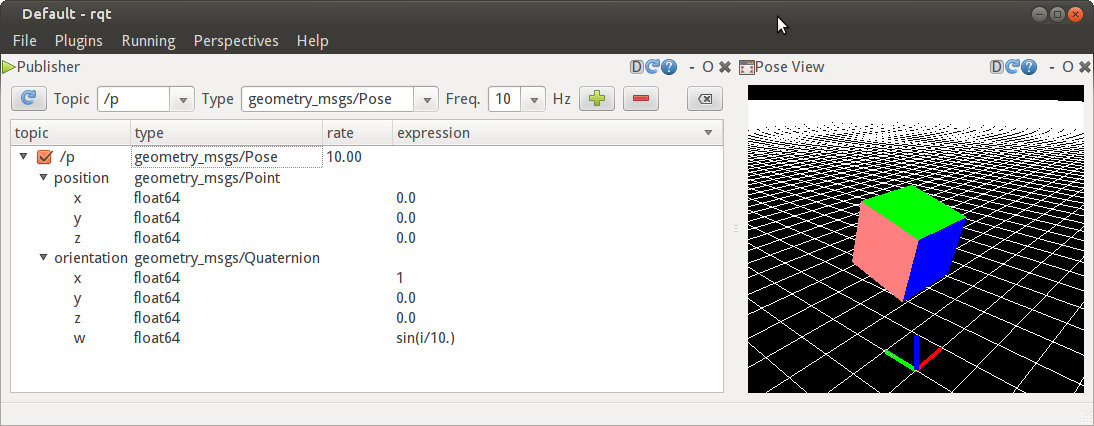
\includegraphics[height=6cm,width=1\textwidth,keepaspectratio]{rqt_pose_view.png}
                % \caption{caption_name}
                \label{fig:rqt_pose_view.png}
             \end{figure}
        \end{column}
    \end{columns}
\end{frame}

\begin{frame}[t]{RViz 2: 3D Visualization}
    \framesubtitle{The Robot's Eye}
    \textbf{When to use:} Viewing spatial data. "What does the robot see?"
    
    \begin{itemize}
        \item \textbf{TF (Transforms):} Coordinate frames relationship (Base $\rightarrow$ Camera).
        \item \textbf{Displays:} LaserScan, PointCloud2, RobotModel (URDF), Map, Odometry.
    \end{itemize}

    \begin{center}
        \begin{figure}[H]
            \centering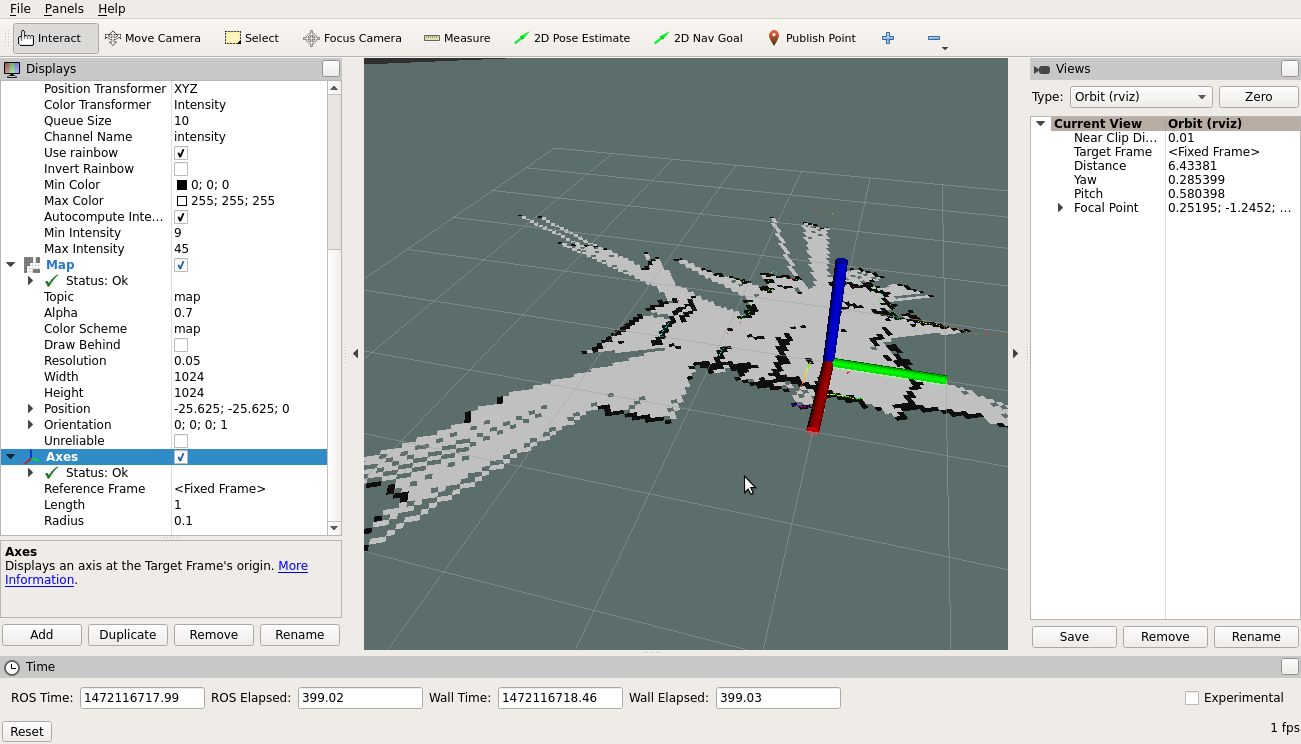
\includegraphics[height=3.5cm,width=1\textwidth,keepaspectratio]{rviz2.png}
            % \caption{caption_name}
            \label{fig:rviz2.png}
        \end{figure}
    \end{center}
\end{frame}

\begin{frame}{References: Tools}
    \begin{enumerate}
        \item [EN] \href{https://docs.ros.org/en/humble/Tutorials/Beginner-CLI-Tools/Introducing-Turtlesim/Introducing-Turtlesim.html}{Turtlesim \& RQT}
        \item [EN] \href{http://wiki.ros.org/rviz}{RViz (ROS1 Wiki but relevant concepts)}
    \end{enumerate}
\end{frame}


\section{Data: Rosbags \& Datasets}

\begin{frame}{What is a Rosbag?}
    \framesubtitle{The Black Box}
    \textbf{Concept:} A rosbag records the \textit{exact} stream of messages passing through topics.
    
    \begin{itemize}
        \item \textbf{Serialization:} Messages are stored in binary format (CDR).
        \item \textbf{Storage:} 
        \begin{itemize}
            \item \textbf{SQLite3:} Default. Single file (or split). Good for compatibility.
            \item \textbf{MCAP:} New standard. Optimized for robotics (indexing, attachments). 
        \end{itemize}
    \end{itemize}
\end{frame}

\begin{frame}{Bags vs Datasets}
    \framesubtitle{Raw vs Cooked}
    \begin{columns}
        \begin{column}{0.48\textwidth}
            \textbf{Rosbag (Raw Log)}
            \begin{itemize}
                \item Contains EVERYTHING (timing, latency).
                \item Unstructured (just topics).
                \item Used for: \textit{Simulated Replay}, Debugging "why did it crash?".
            \end{itemize}
        \end{column}
        \begin{column}{0.48\textwidth}
            \textbf{Dataset (Curated)}
            \begin{itemize}
                \item Extracted from bags (Images, CSV).
                \item Annotated (Labels added).
                \item Used for: \textit{Machine Learning Training}.
            \end{itemize}
        \end{column}
    \end{columns}
\end{frame}

\begin{frame}{Workflow \& Tools}
    \textbf{1. Record:}
    \texttt{ros2 bag record -o output\_name /image /scan}
    
    \textbf{2. Info:}
    \texttt{ros2 bag info output\_name} (Duration, Size, Message count).

    \textbf{3. Visualization:}
    \begin{itemize}
        \item \textbf{Foxglove Studio:} Modern web-based visualizer for MCAP/Bags.
        \item \textbf{PlotJuggler:} Great for analyzing time-series data.
    \end{itemize}
\end{frame}

\begin{frame}{References: Data}
    \begin{enumerate}
        \item [EN] \href{https://docs.ros.org/en/humble/Tutorials/Beginner-CLI-Tools/Recording-And-Playing-Back-Data/Recording-And-Playing-Back-Data.html}{Recording and Playback (Official)}
        \item [EN] \href{https://mcap.dev/}{MCAP File Format}
        \item [EN] \href{https://foxglove.dev/}{Foxglove Studio}
    \end{enumerate}
\end{frame}


\begin{frame}{Launch System}
    \framesubtitle{Writing scripts to run scripts}
    Imagine you have 10 nodes. You don't want 10 terminals.
    
    \textbf{ROS 2 Launch (Python):}
    \begin{itemize}
        \item \textbf{Introspection:} It's python code, so you can use logic (if/else).
        \item \textbf{Events:} Restart node if it crashes.
        \item \textbf{Composition:} Include other launch files (`include\_launch\_description`).
    \end{itemize}
\end{frame}

\begin{frame}[fragile]{Example Launch File}
    \scriptsize
    \begin{columns}[T]
        \begin{column}{0.48\textwidth}
\begin{lstlisting}[language=Python]
from launch import LaunchDescription
from launch_ros.actions import Node

def generate_launch_description():
    return LaunchDescription([
        Node(
            package='my_pkg',
            executable='talker',
            name='my_talker',
            parameters=[{'speed': 5.0}],
            remappings=[('/topic', '/chatter')]
        ),
\end{lstlisting}
        \end{column}
        \begin{column}{0.48\textwidth}
\begin{lstlisting}[language=Python]
        Node(
            package='my_pkg',
            executable='listener',
            name='my_listener'
        )
    ])
\end{lstlisting}
        \end{column}
    \end{columns}
\end{frame}

\begin{frame}{References: Launch}
    \begin{enumerate}
        \item [EN] \href{https://docs.ros.org/en/humble/Tutorials/Intermediate/Launch/Launch-Main.html}{Launch System (Official)}
        \item [EN] \href{https://docs.ros.org/en/humble/How-To-Guides/Launch-file-different-formats.html}{Python vs XML vs YAML Launch}
    \end{enumerate}
\end{frame}

\begin{frame}[t]{General References}
\framesubtitle{}
    \begin{itemize}
        \item \href{https://gitlab.com/ApexAI/autowareclass2020/-/tree/master/lectures/02_ROS2_101}{Autoware class about ROS2}
        \item \href{https://f24.ros.santoslab.org/lectures/}{Intro to ROS2 course}
        \item \href{https://stepik.org/course/221157/promote}{ROS2 курс на степике (русский)}
    \end{itemize}
\end{frame}

\fbckg{fibeamer/figs/last_page.png}
\frame[plain]{}

\end{document}